\chapter{Introduction}

\section{Motivations et modèle}

\subsection{Motivations et résultats précédents}
Ce stage s'inscrit dans l'étude des moyens de transport en libre service tel \emph{Vélib'} ou \emph{Autolib'} à Paris. Le principe est le suivant : un utilisateur prend un véhicule dans n'importe quelle station et se déplace jusqu'à une n'importe quelle station où il dépose son véhicule. Un des problèmes auquel est confronté ce service est le taux de foisonnement, c'est-à-dire le fait que chaque station doit garder un bon équilibre entre le nombre de places et le nombre de véhicule. L'étude de ce rééquilibrage sous certaines hypothèses a fait l'objet de recherche et certains résultat ont déjà été publiés.
\\

Dans l'article \cite{Benchimol2011}, les auteurs ont introduit une version du \emph{C-delivery TSP}\footnote{littéralement, problème du voyageur de commerce avec livraison et une capacité de transport égale à $C$} défini par Chalasani et Motwani dans l'article \cite{Chalasani1999}. Le modèle utilisé est nommé \emph{Static Stations Balancing Problem} abrégé SSBP. Ce modèle s'appuie sur un graphe connexe dans lequel un véhicule (que nous appelerons le \emph{camion} dans la suite) déplace les véhicules en libre service (que nous nommerons \emph{vélos}) d'un sommet à un autre. Le camion peut transporter un nombre fini et maximal $C$ de vélos, en déposer tout ou une partie à chaque sommet et en prendre dans la limite de sa capacité. L'objectif est de trouver le plus court trajet du camion rééquilibrant le graphe.

Les auteurs ont montré que dans le cas général (capacité $C$ et graphe quelconque), le problème était NP-difficile. Cependant, dans le cas du graphe complet avec des coûts unitaires, ils ont pu obtenir un algorithme donnant une solution au plus deux fois plus coûteuse que la solution optimale. Ils ont également décrit une borne inférieure du coût de la solution optimale. Enfin, si le graphe est un arbre, ils ont exhibé un algorithme linéaire donnant le coût d'une solution optimale et le premier mouvement d'une telle solution.
\\

Les auteurs ont également laissé plusieurs questions ouvertes. En particulier, la complexité du rééquilibrage dans le cas où le graphe est un cercle (par exemple des stations le long d'une route entourant un parc) est à ce jour non résolue. Cette question particulière est l'objet de ce stage.

\subsection{Notations et outils}

Soient $F$ un ensemble fini et $H$ un semi-groupe additif. Soit $w \in H^F$. Alors, pour tout sous-ensemble $F'$ de $F$, on note $$w(F') = \sum_{f \in F'} w(f)$$

Soit $G=(V,E)$ un graphe. Pour tout sous-ensemble de sommet $U$ de $V$, on note $\delta(U)$ l'ensemble des arêtes ayant exactement un sommet dans $U$. Par abus de notation, si $v$ est un sommet, on notera $\delta(v)$ au lieu de $\delta(\{v\})$.

Soit $G=(V,E)$ un graphe circulaire. Soit $e \in E$ une arête du graphe. On définit un sens positif dans le graphe. Pour $i \in \ZZ$, on notera $e+i$ la $i^{ème}$ arête $f \in E$ suivant $e$ dans le graphe. (Voir figure \ref{Notation orientation graphe circulaire}.)
\begin{figure}[ht]
  \centering
  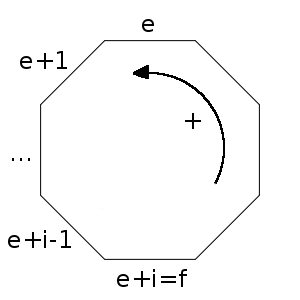
\includegraphics[scale=0.5]{GrapheCirculaire_NotationOrientation.jpg}
  \caption{Orientation du graphe circulaire et ordre des arêtes}
  \label{Notation orientation graphe circulaire}
\end{figure}

Muni d'une telle orientation, pour $u,v \in V$, on définit $\left[ u,v \right]_+$ (resp. $\left[ u,v \right]_-$) l'ensemble des stations rencontrées entre $u$ et $v$ en parcourant $G$ dans le sens positif (resp. négatif). \`A la manière des intervalles, on ouvrira ou fermera les crochets pour exprimer si l'on exclut ou inclut les bornes. (Voir figure \ref{Notation intervalle graphe}.)
\begin{figure}[ht]
  \centering
  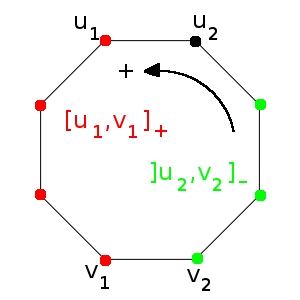
\includegraphics[scale=0.5]{GrapheCirculaire_NotationIntervalle.jpg}
  \caption{Orientation du graphe circulaire et notation sous forme d'intervalle}
  \label{Notation intervalle graphe}
\end{figure}

Pour $X,Y \subseteq V$, on notera $E[X:Y]$ l'ensemble des arêtes ayant un sommet dans $X$ et un sommet dans $Y$ et tel que leur deux sommets soient dans $X \cup Y$. Par soucis de concision, on notera $E[X] = E[X:Y]$.

\subsection{Modèle}

On se donne un graphe $G=(V,E)$ et une capacité $C \ge 0$. Un \emph{état} $s$ est un couple $(\bs{x},p)$ où $\bs{x} \in \RR^V_+$ et $p$ est une arête dans $V$. Deux états $s=(\bs{x},p)$ et $s'=(\bs{y},q)$ sont dits \emph{adjacents} s'ils ont simultanément :
\begin{itemize}
\item $x_v=y_v$ pour tout $v \notin \{p,q\}$ ;
\item $pq \in E$ ;
\item $x_p-y_p = y_q-x_q$ ;
\item $\left| x_p-y_p \right| \le C$.
\end{itemize}

Un mouvement consiste à aller d'un état $s$ à un état adjacent $s'$. Si le graphe est doté par un coût $\bs{c} \in \RR^E_+$, le coût d'un mouvement entre deux états adjacents $s=(\bs{x},p)$ et $s'=(\bs{y},q)$ est simplement $c(pq)$. Le coût d'une séquence de mouvement est la somme des coût des mouvement de la séquence.
\\

Il est facile de voir que l'état $s=(\bs{x},p)$ code la position $p$ du camion et le nombre $x_v$ de vélos sur chaque stations $v$. Un mouvement correspond bien à un mouvement réel du camion pendant lequel il transorte $x_p-y_p$ vélos de la stations $p$ à la sation $q$.

Dans notre étude, le problème consiste à aller d'un état initial $i=(\bs{x},p)$ à un état cible $t=(\bs{y},q)$ en utilisant que des mouvements entre des états adjacents et avec une séquence de coût minimal.

Nous dirons qu'un sommet $v$ (ou une station) est \emph{en excès} (resp. \emph{en défaut}) si $x_v > y_v$ (resp. $x_v < y_v$). Une station sera dite \emph{équilibrée} si $x_v=y_v$. L'ensemble des stations équlibrées sera noté $B(\bs{x},\bs{y})$.
\\
La même notion peut être étendue à un sous-ensemble de sommets : $U \subseteq V$ est dit en excès (resp. en défaut, équilibré) si $x(U) > y(U)$ (resp. $x(U) < y(U)$, $x(U) = y(U)$).

Pour une séquence de mouvements, pour chaque arête $e \in E$, on notera $z_e$ la variable ``comptant'' le nombre de fois où le camion est passé par l'arête $e$.

Dans l'ensemble de cette étude, nous supposerons également que $x(V) = y(V)$ sinon le problème n'a pas de solutions. En outre, nous supposerons toujours que le graphe possède au moins 3 sommets.
\\

Le problème introduit par les auteurs de l'article \cite{Benchimol2011} s'exprime de la manière qui suit.
\\
\\
\textbf{Données.} Un graphe $G=(V,E)$, une fonction de coût $\bs{c} \in \RR^E_+$, une capacité $C$ et deux états $i=(\bs{x},p)$ (état initial) et $t=(\bs{y},q)$ (état cible).
\\
\textbf{Tâche.} Trouver le coût minimal $\Upsilon_{G}$ de la séquence de mouvements permettant d'aller de l'état $i$ à l'état $t$ et le premier mouvement d'une telle séquence.

\section{Résultats}

La section \ref{Résultats préliminaires} présentent les hypothèses de travail et quelques résultats préliminaires sur les graphes circulaires à $n$ sommets. La section \ref{Cas du Triangle} présente un algorithme permettant d'obtenir une solution optimale avec au plus cinq disjonctions de cas dans le cas du triangle ainsi qu'une preuve de l'optimalité de la solution retournée par l'agorithme. La section \ref{Capacité infinie} présente un algorithme polynomial permettant d'obtenir une solution optimale dans le cas où le camion peut transporter une infinité de vélos et où $p=q$ et sa preuve. La section \ref{Capacite unitaire} présente quelques pistes concernant la capacité unitaire mais ne démontre pas d'algorithme.